\chapter*{前言}
\addcontentsline{toc}{chapter}{王汝梅《新刻繡像批評金瓶梅》前言}
\markboth{\titlename}{前言}

\begin{declareqianyan}
王汝梅\qquad\ 
\end{declareqianyan}	

《金瓶梅》是我國小說史上第一部文人獨立創作的長篇白話世情小說,對後世的小說創作與文化嬗變產生過較大影響,在文學史、文化史上具有重要地位。近年來,我國《金瓶梅》研究不斷取得新的進展,引起國外漢學家的注意。人民文學出版社出版的《金瓶梅詞話》刪節本,齊魯書社出版的《張竹坡批評第一奇書金瓶梅》刪節本,香港星海文化出版有限公司出版的《金瓶梅詞話》全校本,都促進了《金瓶梅》研究的深入發展。

《金瓶梅》的版本,大體上可分為兩個系統,三種型別。一是詞話本系統,即《新刻金瓶梅詞話》,現存三部完整刻本及一部二十三回殘本(北京圖書館藏本、日本日光山輪王寺慈眼堂藏本、日本德山毛利氏栖息堂藏本及日本京都大學附屬圖書館藏殘本)。二是崇禎本系統,即《新刻繡像批評金瓶梅》,現存約十五部(包括殘本、抄本、混合本)。第三種型別是張評本,即《張竹坡批評第一奇書金瓶梅》,屬崇禎本系統,又與崇禎本不同。在兩系三類中,崇禎本處於《金瓶梅》版本流變的中間環節。它據詞話本改寫而成,又是張評本據以改易、評點的祖本,承上啟下,至關重要。現存的崇禎本都十分珍貴,一般不易見到,因此,把存世的主要崇禎本全面地校勘一下,出版一部會校本《新刻繡像批評金瓶梅》,就顯得十分重要了。它不僅有助於認識《金瓶梅》的版本系統,而且也是探討《金瓶梅》成書之謎、作者之謎,研究作品思想藝術價値的客觀依據,是《金瓶梅》研究的基礎工程。

\subsection*{一、崇禎諸本的特徵、類別及相互關係}

刊刻於十卷本《金瓶梅詞話》之後的《新刻繡像批評金瓶梅》,是二十卷一百回本。卷首有東吳弄珠客《金瓶梅序》。書中有插圖二百幅,有的圖上題有刻工姓名,如劉應祖、劉啟先、黃子立、黃汝耀等。這些刻工活躍在天啟、崇禎年間,是新安(今安徽歙縣)木刻名手。這種刻本避明崇禎帝朱由檢諱。根據以上特點和刻本的版式字型,一般認為這種本子刻印在崇禎年間,因此簡稱為崇禎本,又稱繡像本或評改本。

現仍存世的崇禎本(包括清初翻刻的崇禎系統版本)有十幾部,各部之間大同略有小異。從版式上可分為兩大類。一類以北京大學圖書館藏本為代表,書每半葉十行,行二十二字,扉頁失去,無廿公跋,回首詩詞前有「詩曰」或「詞曰」二字。日本天理圖書館藏本、上海圖書館藏甲乙兩本、天津圖書館藏本、殘存四十七回本等,均屬此類。另一類以日本內閣文庫藏本為代表,書每半葉十一行,行二十八字,有扉頁,扉頁上題《新鐫繡像批評原本金瓶梅》,有廿公跋,回首詩詞前多無 「詩曰」或「詞曰」二字。首都圖書館藏本、日本京都大學東洋文化研究所藏本屬於此類。

崇禎諸本多有眉批和夾批。各本眉批刻印行款不同。北大本、上圖甲本以四字一行居多,也有少量二字一行的。天圖本、上圖乙本以二字一行居多,偶有四字一行和三字一行的。內閣本眉批三字一行。首圖本有夾批無眉批。

為了清理崇禎諸刻本之間的關係,需要先對幾種稀見版本作一簡單介紹:

{\large\kaishu{王孝慈舊藏本}}。王孝慈為書畫家,通縣人,原藏《新刻繡像批評金瓶梅》插圖二冊,二百幅。一九三三年北平古佚小說刊行會版詞話本中的插圖,即據王氏藏本影印。圖甚精致,署刻工姓名者多。第一回第二幅圖「武二郎冷遇親哥嫂」欄內右側題署「新安劉應祖鐫」六字,為現存其他崇禎本插圖所無。其第一回回目「西門慶熱結十弟兄」,現存多數本子與之相同,僅天圖本、上圖乙本略異。從插圖和回目判斷,王氏藏本可能是崇禎系統的原刻本。

{\large\kaishu{殘存四十七回本}}。近年新發現的。扉頁右上題「新鐫繡像批評原本」,中間大字「金瓶梅」,左題「本衙藏版」。插圖有九十幅,第五回「飲鴆藥武大遭殃」及第二十二回「蕙蓮兒偸期蒙愛」,俱題署刻工劉啟先姓名。此殘本版式、眉批行款與北大本相近,卷題也與北大本相同,但扉頁則依內閣本所謂「原本」扉頁格式刻印。此版本兼有兩類本子的特徵,是較晚出的版本,大約刊印在張評本刻印前的順治或康熙初年,流傳至張評本刊印之後。該書流傳中失去五十三回,用張評本配補,成了崇禎本和張評本的混合本。從明末至清中葉,《金瓶梅》由詞話本、崇禎本同步流傳演變為崇禎本和張評本同步流傳,其遞變端倪,可由此本看出。

{\large\kaishu{吳曉鈴先生藏抄本}}。四函四十冊,二十卷百回,是一部書品闊大的烏絲欄大字抄本。抄者為抄本刻制了四方邊欄、行間夾線和書口標「金瓶梅」的木版。吳先生云:「從字型風格看來,應屬乾隆前期。」書中穢語刪除,無眉批夾批。在崇禎諸本的異文處,此本多與北大本相同,但也有個別地方與北大本不同。由此看來,此本可能系據崇禎系統原刊本抄錄,在研究崇禎本流變及版本校勘上,頗有價値。

{\large\kaishu{《繡刻古本八才子詞話》}}。吳曉鈴先生云:「順治間坊刻《繡像八才子詞話》,大興傅氏碧蕖館舊藏。今不悉散佚何許。」(《金瓶梅詞話最初刊本問題》)吳先生把此一種本子視為清代坊間刊詞話本。美國韓南教授着錄:「扉頁題《繡刻古本八才子詞話》,其下有『本衙藏版』等字。現存五冊:序文一篇、目錄,第一、二回,第十一至十五回,第三十一至三十五回,第六十五至六十八回。序文年代順治二年(一六四五),序者不詳。十卷百回。無插圖。」(《金瓶梅的版本及其他》)韓南把它列入崇禎本系統。因韓南曾借閱傅惜華藏書,筆者採取韓南的意見,把此版本列入崇禎系統。

{\large\kaishu{周越然舊藏本}}。周越然着錄:「新刻繡像批評金瓶梅二十卷百回。明崇禎間刊本,白口,不用上下魚尾,四周單欄,每半頁十行,每行二十二字,眉上有批評,行間有圈點。卷首有東吳弄珠客序三葉,目錄十葉,精圖一百葉。此書版刻、文字均佳。」據版式特徵應屬北大本一類,與天圖本、上圖乙本相近或同版。把現存周越然舊藏本第二回圖「俏潘娘簾下勾情」影印件與北大本圖對勘,北大本圖左下有 「黃子立刊」四字,周藏本無(右下有周越然章)。

根據上述稀見版本的着錄情況和對現存崇禎諸本的考查,我們大體上可以判定,崇禎系統內部各本之間的關係是這樣的:目前僅存插圖的通州王氏舊藏本為原刊本或原版後印本。北大本是以原刊本為底本翻刻的,為現存較完整的崇禎本。以北大本為底本翻刻或再翻刻,產生出天理本、天圖本、上圖甲乙本、周越然舊藏本。對北大本一類版本稍作改動並重新刊印的,有內閣本、東洋文化研究所本、首圖本。後一類版本卷題作了統一,正文文字有改動,所改之處,多數是恢復了詞話本原字詞。在上述兩類崇禎本流傳之後,又刊刻了殘存四十七回本,此本兼有兩類版本的特徵。為使讀者一目了然,特將所知見諸本關係,列表如下:
{\clearpage}
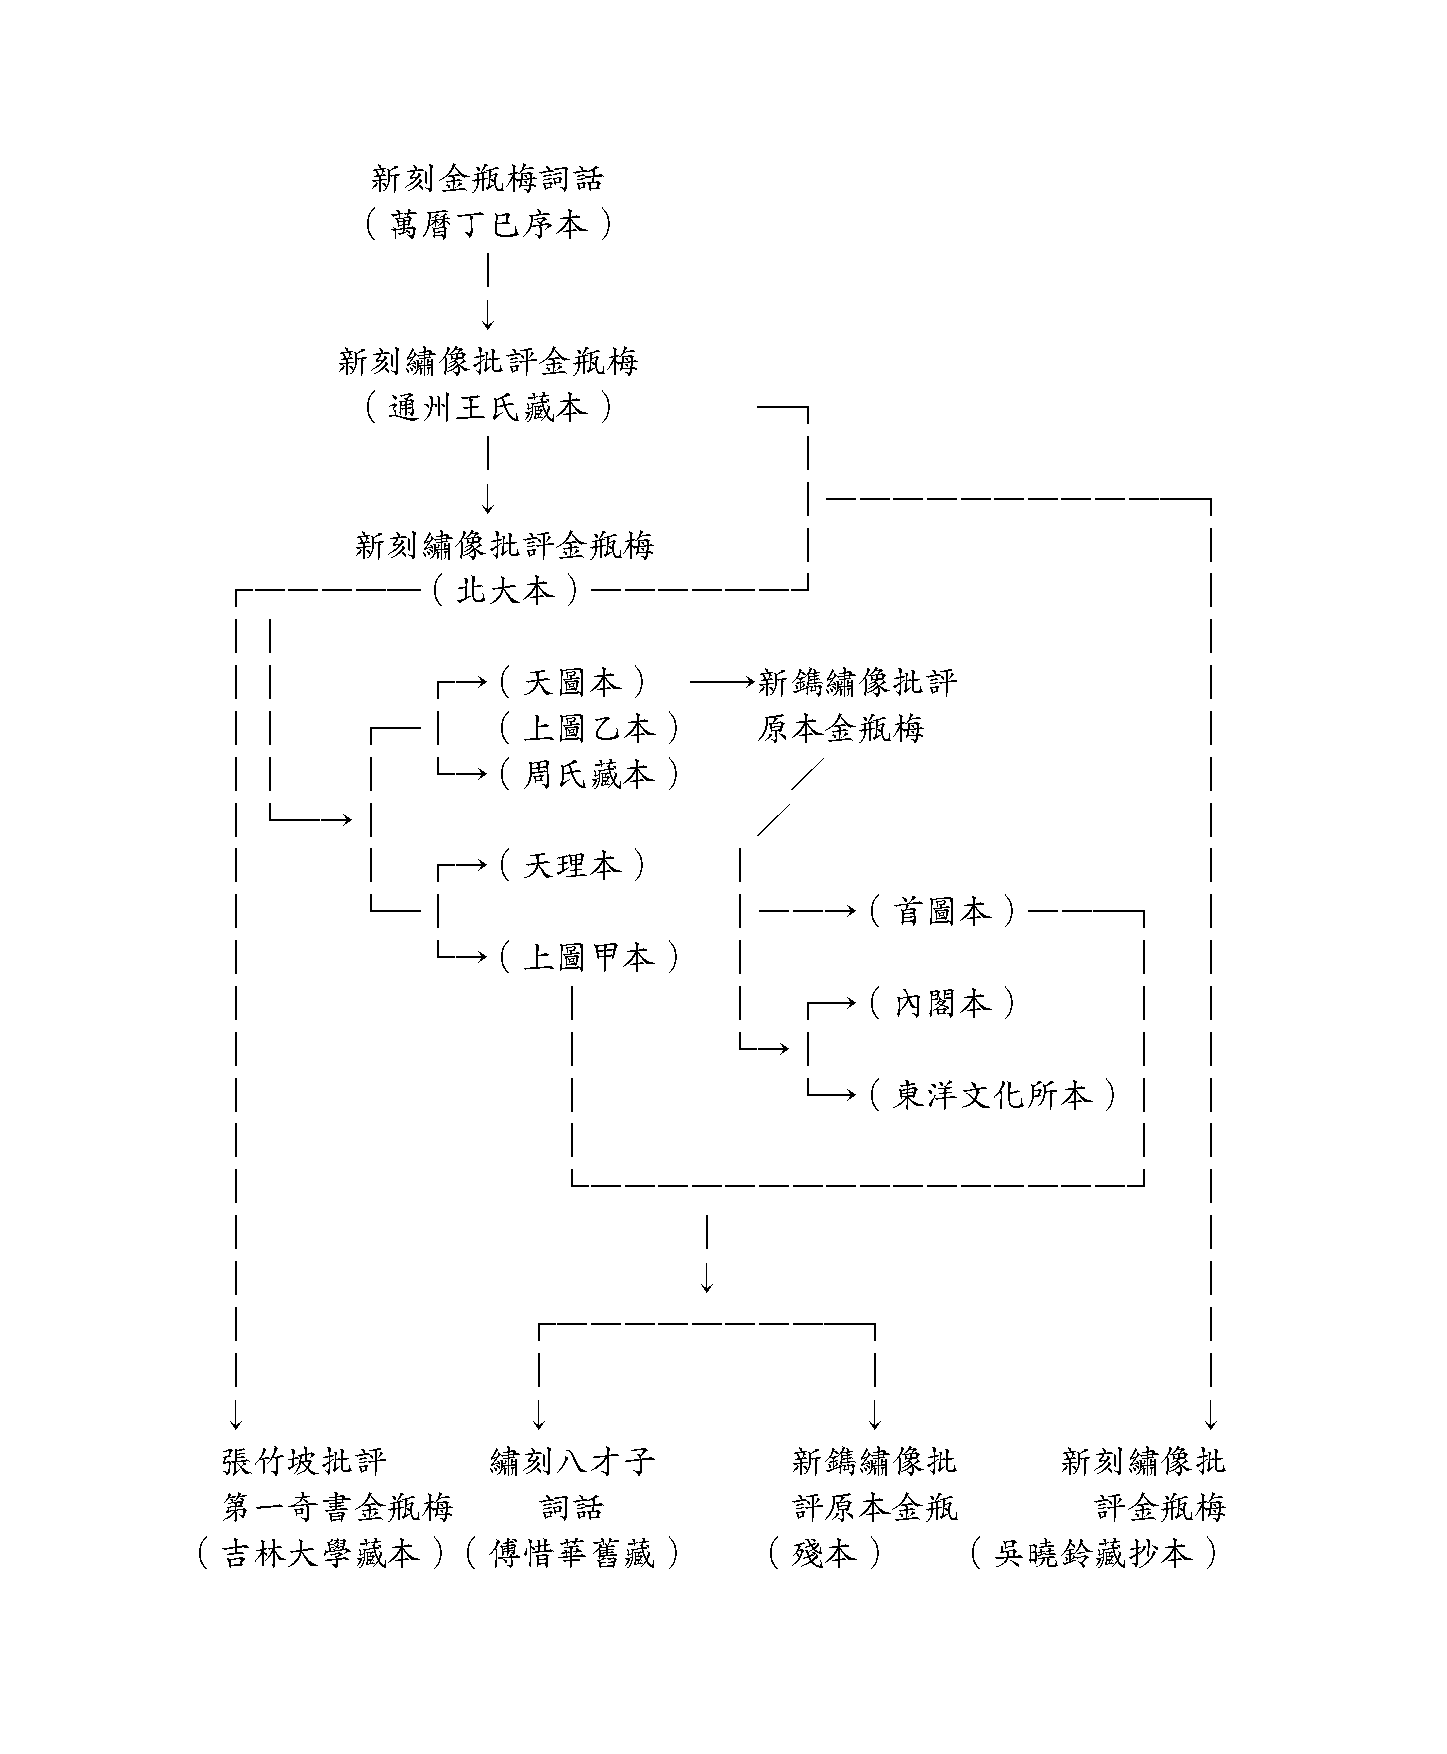
\includepdf[pages={1},fitpaper=false]{version_relations.pdf}

\subsection*{二、崇禎本和萬曆詞話本的關係}

崇禎本與萬曆詞話本相同又相異,相異而又相關。茲就崇禎本與萬曆詞話本明顯的相異之處,考查一下二者之間的關係。

(一)改寫第一回及不收欣欣子序。崇禎本把第一回「景陽岡武松打虎」改為「 西門慶熱結十弟兄」。從開首到「知縣陞堂,武松下馬進去」,是改寫者手筆,以 「財色」論作引子,寫至十弟兄在玉皇廟結拜。文句中有「打選衣帽光鮮」、「看飯來」、「哥子」、「千百斤水牛般氣力」等江浙習慣用語。「武松下馬進去」以後,文字大體與詞話本同,刪減了「看顧」、「叉兒難」等詞語。改寫後,西門慶先出場,然後是潘金蓮嫌夫賣風月,把原來武松為主、潘金蓮為賓,改成了西門慶、潘金蓮為主、武松為賓。改寫者對《金瓶梅》有自己的看法,他反對欣欣子的觀點,因此把詞話本中與欣欣子序思想一致的四季詞、四貪詞、引子,統統刪去了。

欣欣子序闡述了三個重要觀點:第一、《金瓶梅傳》作者是「寄意於時俗,蓋有謂也。」第二、《金瓶梅傳》是發憤之作,作者「爰罄平日所蘊者,着斯傳」。第三、《金瓶梅傳》雖「語涉俚俗,氣含脂粉」,但不是淫書。欣欣子冲破儒家詩教傳統,提出不要壓抑哀樂之情的進步觀點。他說:「富與貴,人之所慕也,鮮有不至於淫者;哀與怨,人之所惡也,鮮有不至於傷者。」這種觀點與李贄反對「矯強」、主張「自然發於性情」的反禮教思想是一致的。崇禎本改寫者反對這種觀點,想用「財色」論、「懲戒」說再造《金瓶梅》,因此他不收欣欣子序。而東吳弄珠客序因觀點與改寫者合拍,遂被刊為崇禎本卷首。

(二)改寫第五十三、五十四回。崇禎本第五十三、五十四兩回,與詞話本大異小同。詞話本第五十三回「吳月娘承歡求子息,李瓶兒酬願保官哥」,把月娘求子息和瓶兒保官哥兩事聯絡起來,圍遶西門慶「子嗣」這一中心展開情節,中間穿插潘金蓮與陳經濟行淫、應伯爵為李三、黃四借銀。崇禎本第五十三回「潘金蓮驚散幽歡,吳月娘拜求子息」,把潘金蓮與陳敬濟行淫描寫加濃,並標為回目,把李瓶兒酬願保官哥的情節作了大幅度刪減。改寫者可能認為西門慶不信鬼神,所以把灼龜、劉婆子收驚、錢痰火拜佛、西門慶謝土地、陳經濟送紙馬等文字都刪去了。崇禎本第五十四回把詞話本劉太監庄上河邊郊園會諸友,改為內相陸地花園會諸友,把瓶兒胃虛血少之病,改為下淋不止之病。瓶兒死於血山崩,改寫者可能認為血少之症與結局不相符而改。上述兩回,儘管文字差異較大,內容亦有增有減,但基本情節並沒有改變,仍可以看出崇禎本是據萬曆詞話本改寫而成,並非另有一種底本。

値得注意的是,詞話本第五十三、五十四兩回與前後文脈絡貫通,風格也較一致,而崇禎本這兩回卻描寫粗疏,與前後文風格亦不太一致。例如讓應伯爵當西門慶面說:「只大爹他是有名的潘驢鄧小閑不少一件」,讓陳敬濟偸情時扯斷潘金蓮褲帶,都顯然不符合人物性格,手法拙劣。

(三)崇禎諸本均避崇禎皇帝朱由檢諱,詞話本不避。如詞話本第十七回「則虜患何由而至哉!」、「皆由京之不職也」,崇禎本改「由」為「繇」;第九十五回 「巡檢司」、「吳巡檢」,崇禎本改「檢」為「簡」。此一現象亦說明崇禎本刊刻在後,並系據詞話本而改。

(四)崇禎本在版刻上保留了詞話本的殘存因素。北大本第九卷題作「新刻繡像批點金瓶梅詞話卷之七」,這是崇禎本據詞話本改寫的直接證明。此外,詞話本誤刻之字,崇禎本亦徃徃相沿而誤。如詞話本第五十七回:「我前日因徃西京」,「 西京」為「東京」之誤刻,崇禎本相沿;詞話本第三十九回:「老爹有甚釣語分付 」,「釣」為「鈞」之誤刻,北大本、內閣本亦相沿。上述殘存因素,可以看作是崇禎本與其母體《新刻金瓶梅詞話》之間的臍帶。

(五)其他相異之處:崇禎本刪去詞話本第八十四回吳月娘為宋江所救一段文字;崇禎本改動詞話本中部分情節;崇禎本刪去詞話本中大量詞曲;崇禎本刪減或改動了詞話本中的方言語詞;崇禎本改換了詞話本的回首詩詞;崇禎本比詞話本回目對仗工整;等等。

大量版本資料說明,崇禎本是以萬曆詞話本為底本進行改寫的,詞話本刊印在前,崇禎本刊印在後。崇禎本與詞話本是母子關係,而不是兄弟關係。

崇禎本刊印前,也經過一段傳抄時間。謝肇淛就提到二十卷抄本問題。他在《金瓶梅跋》中說:「書凡數百萬言,為卷二十,始末不過數年事耳。」這篇跋,一般認為寫於萬曆四十四年至四十六年(一六一六——一六一八)。這時謝肇淛看到的是不全的抄本,於袁宏道得其十三,於丘諸城得其十五。看到不全抄本,又云「為卷二十」,說明謝已見到回次目錄。二十卷本目錄是分卷次排列的。這種抄本是崇禎本的前身。設計刊刻十卷詞話本與籌劃改寫二十卷本,大約是同步進行的。可能在刊印詞話本之時即進行改寫,在詞話本刊印之後,以刊印的詞話本為底本完成改寫本定稿工作,於崇禎初年刊印《新刻繡像批評金瓶梅》。繡像評改本的改寫比我們原來想象的時間要早些。但是,崇禎本稿本也不會早過十卷本的定型本。蒲安迪教授認為,崇禎本的成書時間應「提前到小說最早流傳的朦朧歲月中,也許甚至追溯到小說的寫作年代」(《論崇禎本金瓶梅的評註》),顯然是不妥當的。從崇禎本的種種特徵來看,它不可能與其母本詞話本同時,更不可能早於母本而出生。

\subsection*{三、崇禎本評語在小說批評史上的重要地位}

崇禎本評語是古代小說批評的一宗珍貴遺產。評點者在長篇小說由英雄傳奇向世情小說蛻變的轉折時期,冲破傳統觀念,在李贄、袁宏道的「童心」、「性靈」 、「眞趣」、「自然」的審美新意識啟示下,對《金瓶梅》藝術成就進行了開拓性的評析。評點者開始注重寫實,注重人物性格心理的品鑑,在馮夢龍、金聖嘆、李漁、張竹坡、脂硯齋之前,達到了古代小說批評的新高度。其主要價値有如下幾點:

(一)肯定《金瓶梅》是一部世情書,而非淫書。評點者認為書中所寫人事天理,全為「世情所有」,「如天造地設」。評點者第一次把《金瓶梅》與《史記》相提並論,認為《金瓶梅》「從太史公筆法來」,「純是史遷之妙」。評點者批判了淫書論,他說:「讀此書而以為淫者、穢者,無目者也。」明末《金瓶梅》評論有三派觀點。第一,從進步文藝思潮出發,對《金瓶梅》的產生表示驚喜、贊賞,以欣欣子、袁宏道、謝肇淛為代表。第二,接受進步思潮影響,又受傳統觀念束縛,對此書持又肯定又否定態度,認為此書是淫書、穢書,所以要刊印,蓋為世戒,非為世勸,以東吳弄珠客為代表。第三,固守傳統觀念,持全盤否定看法,認為此書淫穢,壞人心術,決當焚之,以董思白為代表。崇禎本評點者鮮明地批評了第二、第三兩種觀點。

(二)分析了《金瓶梅》中衆多人物的複雜性格。魯迅曾指出,《紅樓夢》的可貴之處在於它突破了我國小說人物塑造中「叙好人完全是好,壞人完全是壞」的傳統格局。其實,最早突破這一格局的應該是《金瓶梅》。《金瓶梅》已經擺脫了傳統小說那種簡單化的平面描寫,開始展現眞實的人所具有的複雜矛盾的性格。對於這一點,崇禎本評點者注意到了。他在評析潘金蓮時,既指出她的「出語狠辣」 ,「俏心毒口」,慣於「聽籬察壁」、「愛小便宜」等弱點,也贊美她的「慧心巧舌」、「韻趣動人」等「可愛」之處。評析李瓶兒時,既說她「愚」、「淺」,也指出她「醇厚」、「情深」。即使是西門慶,評點者亦認為作者並非把他寫得絕對的惡,指出「西門慶臨財徃徃有廉恥、有良心」,資助朋友時「脫手相贈,全無吝色」。尤其可貴的是,評點者冲破了封建傳統道德的束縛,對潘金蓮這樣一個「淫婦」,處處流露出贊美和同情。在潘金蓮被殺後,評點者道:「讀至此,不敢生悲,不忍稱快,然而心實惻惻難言哉!」這是對一個複雜形象的充滿矛盾的審美感受。

(三)評析了作者刻畫人物的傳神技巧。評點者說作者「寫笑則有聲,寫想則有形」,「並聲影、氣味、心思、胎骨」俱摹出,「眞爐錘造物之手」。他特別贊賞對潘金蓮的刻畫,說其「撒嬌弄癡,事事堪入畫」,其「靈心利口」,「乖恬」 「可愛」。在四十三回作者寫金蓮喬粧假哭時,評點者道:「倔強中實含軟媚,認眞處微帶戲謔」,點出作者不僅善於描摹人物的聲容笑貌,還能借形傳神,展現人物的內心世界。

(四)崇禎本評語顯示了評點者新的藝術視角。傳統的評論重教化而不重審美,重史實而不重眞趣。評點者冲破這種傳統,從新的藝術視角對《金瓶梅》全面品評。他稱作者為「寫生手」,很多評語肯定作品的寫實特點,白描手法,一再評述作者的藝術眞趣。通俗、眞趣、寫生,這種新和藝術視角,反映了萬曆中後期的美學追求。馮夢龍的「事贗而理眞」論,金聖嘆的性格論,李漁的幻境論,張竹坡的情理論,脂硯齋的「情情」論,使古代小說批評達到成熟與繁榮的高峯,而早於他們的崇禎本評點者,對明清小說批評的發展,可以說起了奠基與開拓的作用。

袁宏道在一六九五年傳遞了《金瓶梅》抄本的第一個資訊,驚訝《金瓶梅》的出現,肯定《金瓶梅》的自然之美。謝肇淛在《金瓶梅跋》中稱此書為「稗官之上乘」,作者為「爐錘之妙手」,特別評述了作者寫人物「不徒俏其貌,且並其神傳之」的特點。崇禎本評點,可以看作是袁宏道、謝肇淛對《金瓶梅》評價具體化的審美反映。


